\section{Experimental Results}



    We evaluated the proposed approach on a dataset consisting of $N = 4$ books in $I = 4$ poses. We used two pairs of books which are ambiguous on the back and unambiguous on the front. \figref{fig:object_dataset} shows the covers of all the books used for the experiment. All poses are presented in \figref{fig:pose_dataset}. 
    
\begin{figure}
\centering
    		
\includegraphics[width = 0.2\columnwidth]{pics/math_cover1_ok.jpg}
    		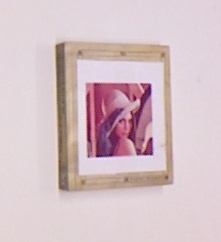
\includegraphics[width = 0.2\columnwidth]{pics/math_cover2_ok.jpg}
    		
\includegraphics[width = 0.2\columnwidth]{pics/first_cover1.jpg}
    		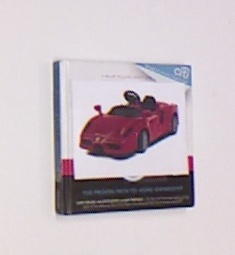
\includegraphics[width = 0.2\columnwidth]{pics/first_cover2.jpg}
    		\caption{Books from the cover side used for the experiment. Two first books and two last books look the same from the back side.}
	\label{fig:object_dataset}
    \end{figure}     
    
    
     \begin{figure}
     \centering
    		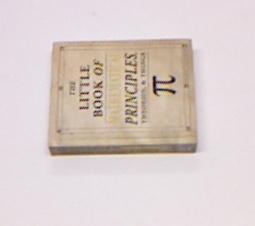
\includegraphics[width = 0.2\columnwidth]{pics/math_cover1.jpg}
    		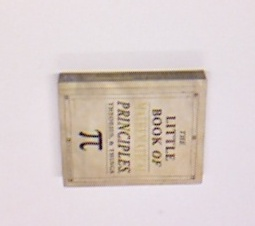
\includegraphics[width = 0.2\columnwidth]{pics/math_cover1_rot.jpg}
    		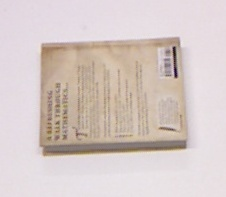
\includegraphics[width = 0.2\columnwidth]{pics/math_down.jpg}
    		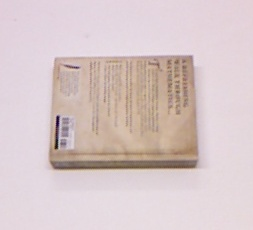
\includegraphics[width = 0.2\columnwidth]{pics/math_down_rot.jpg}
    		\caption{All the poses used for object-pose recognition. Please note the visibility of the spine.}
	\label{fig:pose_dataset}
    \end{figure}       
    
    
$M = 654$ unique features were extracted from a set of ideal images of each object-pose pair. We recorded $100$ training samples for each object-pose pair to learn the likelihood distribution $\prob{f|o,p}$. For the ambiguous cases, we used the same training images.

    Our experimental setup consists of an RGB camera and one of the books. In our preliminary experiment, all the actions were executed by a human.

    \subsection{Object Recognition}
    
	In order to evaluate the object recognition model, we trained the model on $80$ samples and held out $20$ samples for cross validation. The average prediction accuracy for the unambiguous cases is $99.67\%$ for the training data and $93.75\%$ for the cross validation data. We did not include the ambiguous poses in the cross validation results because these ambiguous cases were designed to cause static object recognition to fail. %It is also worth noting that the only errors were confusion between whether the spine was visible or not.
    
 
        
%        \begin{table}[h]
%                \centering
%                \begin{tabular}{|c|c|}
%                \hline
%                Average Training Accuracy & Average Cross Validation Accuracy \\
%                \hline
%                99.67\% & 93.75\% \\
%                \hline
%                \end{tabular}
%                \caption{Average accuracy results for object recognition part of the model.}
%                \label{tab:accuracy}
%		\end{table}

    \begin{figure}
    \centering
    		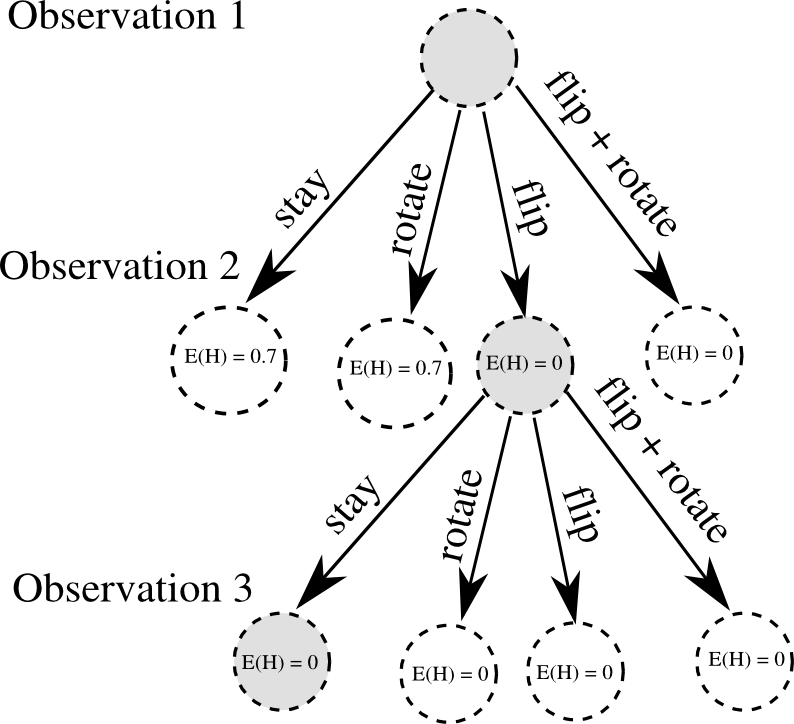
\includegraphics[width = 0.7\columnwidth]{pics/tree_small.png}
    	\caption{Decision tree based on the action selection algorithm. Each node in the tree represents the expected entropy of the posterior probability for a given action. Colored nodes indicate the choice of the action that results in the minimum expected entropy.}
    	    	\label{fig:tree}
    \end{figure}
    
    \begin{figure}
    	    \raisebox{0.5\height}{
\includegraphics[width = 0.39\columnwidth]{pics/obs1.jpg}}
    		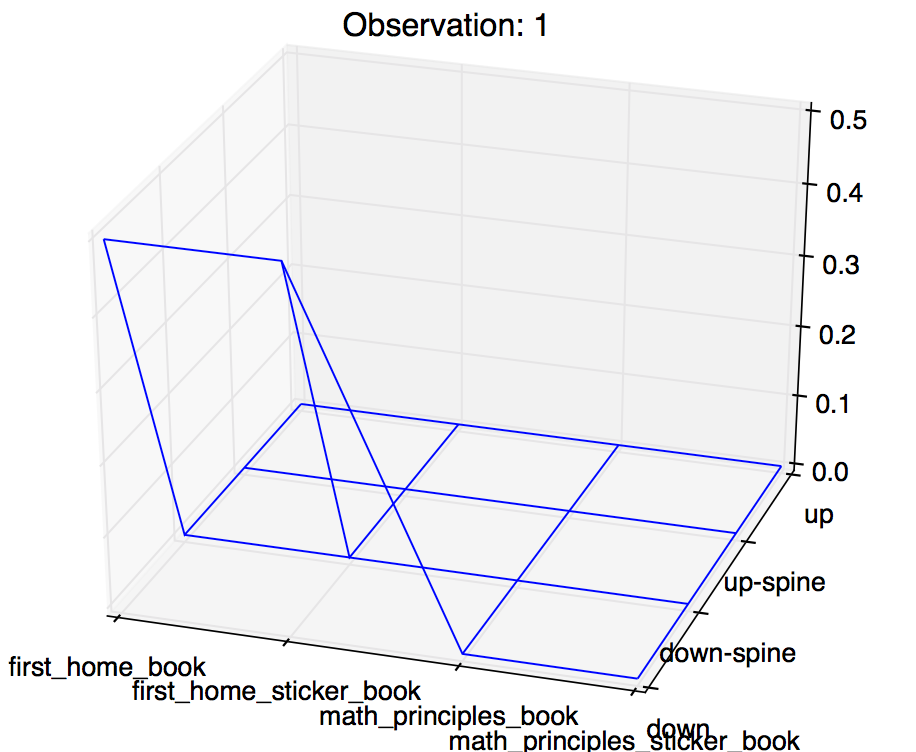
\includegraphics[width = 0.6\columnwidth]{pics/experimentObs1.png}\\
 		\raisebox{0.5\height}{
\includegraphics[width = 0.39\columnwidth]{pics/obs2.jpg}}
    		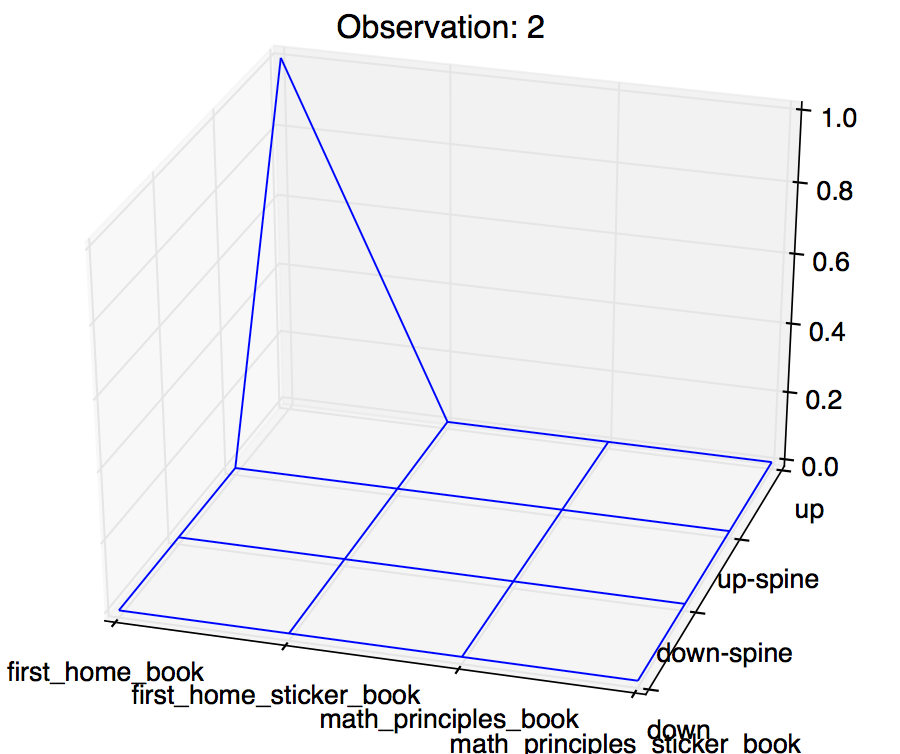
\includegraphics[width = 0.6\columnwidth]{pics/experimentObs2.png}

	\caption{ Top-left: observed image for the first observation. Top-right: Posterior probability of object and pose after the first observation.	Bottom: Analogous graphs after the second observation (i.e. after the action was taken).}
    	\label{fig:posteriors}
    \end{figure}

\vspace{-1ex}
    \subsection{Action Selection}
	An action selection experiment is represented by the decision tree in \figref{fig:tree}.    
	The ambiguous back of the book pose was observed as shown in \figref{fig:posteriors} (top-left). As expected, the posterior probabilities were split between the two ambiguous books shown in \figref{fig:posteriors} (top-right).    

 Of the four actions, staying and rotating result in similarly ambiguous poses resulting in an expected entropy of $0.7$. Flipping the book over, with and without rotating, lead to similarly unambiguous poses with an expected entropy of $0$. After flipping the book, the robot observes the cover (\figref{fig:posteriors} bottom-left) and predicted the correct object with 100\% certainty (\figref{fig:posteriors} bottom-right).

        %The expected entropy is calculated again for each action and they are all $0$, which means that there is no action that will provide the reduction of the expected entropy - the algorithm has converged. %Once the object recognition algorithm has converged to 100\% certainty, the updated posterior will always remain the same as the previous posterior.
    
    
        %The experiment is constructed as follows. We expose an object to the Kinect sensor and obtain the recognition result. In the next step we employ the action selection algorithm to choose the best action and we execute it.~\figref{fig:tree} presents a decision tree that is visualizes the best action actions chosen by the algorithm and the respective observations. In order to measure if the action improved the previous recognition we compute the posterior probability of the object, which is shown together with the respective observation in~\figref{fig:posteriors}. We execute actions until the algorithm converges which means that the action selection algorithm returns says that all the actions do not provide a reduction of expected entropy.

    %\subsection{Discussion}
    % describe the behaviour of posteriors
    % explain why it chose this action
    % explain why we took this exagurated example of the books with stickers
    % show encyclopedia example
    % talk a bit about continous pose    
        

        
        

    
    
    
    
        
        


        %*explain our setup
        % we have a kinect, 4 object, 4 poses each, 50 sift features per object-pose pair
        % 100 training images per object-pose pair
        % we move the object with our hands for now
        %  

        %*assumptions
        % perfect actions (no noise)
        % discrete poses 
        % we see one object at a time
        % we see a known object

        %*explain experiment
        % we show the object to the kinect and recognize it based on our recognition module
        % results for all objects and poses are in the table
        % we figure out the best action (in the table)
        % we check recognition after the action has been taken (in the table)


%        \begin{itemize}
%        \item explain our dataset
%        \item show pictures of objects
%        \item show cross validation results for our training
%        \item explain the setup
%        \item show real data results for object recognition (table)
%        \item discuss the results, emphasize that the action selection works
%        \end{itemize}